\documentclass[a4paper]{article}
%\documentclass[8pt]{report}
%%%%%%%% CREATE DOCUMENT STRUCTURE %%%%%%%%
%% Language and font encodings
\usepackage[english]{babel}
\usepackage[utf8x]{inputenc}
\usepackage[T1]{fontenc}

%\usepackage{subfig}

%% Sets page size and margins
\usepackage[a4paper,top=3cm,bottom=2cm,left=2cm,right=2cm,marginparwidth=1.75cm]{geometry}

%% Useful packages
\usepackage{amsmath}
\usepackage{graphicx}
\usepackage[colorinlistoftodos]{todonotes}
\usepackage[colorlinks=true, allcolors=blue]{hyperref}
%\usepackage{caption}
\usepackage[justification=centering]{caption}
\usepackage{subcaption}
\usepackage{sectsty}
\usepackage{float}
\usepackage{titling} 
\usepackage{blindtext}
\usepackage[square,sort,comma,numbers]{natbib}
\usepackage[colorinlistoftodos]{todonotes}
\usepackage{xcolor}
\usepackage{fancyhdr}
\usepackage{lipsum}

%% definitions 
\definecolor{darkgreen}{rgb}{0.0, 0.4, 0.0}

%% Define your personal info here %%%%%%%%%%%%%%%%%%%%%%%
\newcommand\TPid{1}
\newcommand\TPname{NK-landscape models}
\newcommand\Firstname{Joao Filipe}
\newcommand\Familyname{Costa da Quinta}
\newcommand\Email{Joao.Costa@etu.unige.ch}

%%%%%%%%%%%%%%%%%%%%%%%%%%%%%%%%%%%%%%%%%%%%%%%%%%%%%%%

%%%%%%% Page header %%%%%%
\pagestyle{fancy}
\fancyhf{}
\rhead{TP \TPid: \TPname}
\lhead{\Firstname \Familyname}
\rfoot{Page \thepage}


%%%%%%%% DOCUMENT %%%%%%%%
\begin{document}

%%%% Title Page
\begin{titlepage}

\newcommand{\HRule}{\rule{\linewidth}{0.5mm}} 							% horizontal line and its thickness

\center 
 
% University
\textsc{\LARGE Université de Genève}\\[1cm]

% Document info
\textsc{\Large Metaheuristics for optimization}\\[0.2cm]									% Course Code
\HRule \\[0.8cm]
{ \huge \bfseries TP \TPid : \TPname}\\[0.7cm]								% Assignment
\HRule \\[2cm]
\large
\emph{Author:} \Firstname \; \Familyname\\[0.5cm]		
\emph{E-mail:} {\color{blue}\Email}\\[7cm]		
% Author info
% Author info
{\large \today}\\[2cm]

\includegraphics[width=0.4\textwidth]{images/unige_csd.png}\\[1cm] 	% University logo
\vfill 
\end{titlepage}


% ============================================
% ----------------------------------
\newpage
\section{Introduction}
In this TP we will try to solve the problem of finding the maximum of a given function. Our function represents the landscape of a mountain top, to which we can add more ruggedness by changing the parameters. By having higher ruggedness we should witness higher difficulty in finding the global maximum, as we might tricked by local maximums.\\

\section{Problem}
\subsection{Representation}
To represent our mountain top we will use a simple N-bit string, which makes $\{0,1\}^{N}$ our search space. Let $x$ be a random point in our search space, to check if is a maximum we will use a fitness function $F(x)$, this is the function we would like to maximize.
$$F(x) = \sum^{N-K}_{i = 1} f_{K}(x_{i}, ..., x_{i+K})$$
The difficulty will entirely depend on the value K, in this TP we will set $K = \{0,1,2\}$, varying K will make $F(x)$ easier or harder to maximize. Depending on K, $f_{K}$ will have to consider more or less input possibilities, $\{0,1\}^{K+1}$ to be precise.\\
\begin{itemize}
\item [$K=0$] This is the easiest difficulty, this means that $f_{K}()$ gets only 1 parameter $x_{i}$ at a time, which means that there are $\{0,1\}^{1}$ input possibilities. Therefore there is only one maximum $F(x) = \sum^{N}_{i = 1} f_{0}(x_{i})$.
\item [$K=1$] $f_{K}()$ gets 2 parameters $x_{i}$ at a time, therefore there are $\{0,1\}^{2}$ input possibilities. Which means our mountain top will have multiple mountains or multiple local maximums. $F(x) = \sum^{N-K}_{i = 1} f_{1}(x_{i}, x_{i+1})$.
\item [$K=2$] $f_{K}()$ gets 3 parameters $x_{i}$ at a time, so there are $\{0,1\}^{3}$ input possibilities. It will make it even harder to find the global maximum. $F(x) = \sum^{N-K}_{i = 1} f_{2}(x_{i}, x_{i+1}, x_{i+2})$.
\end{itemize}
\begin{figure}[H]
\center
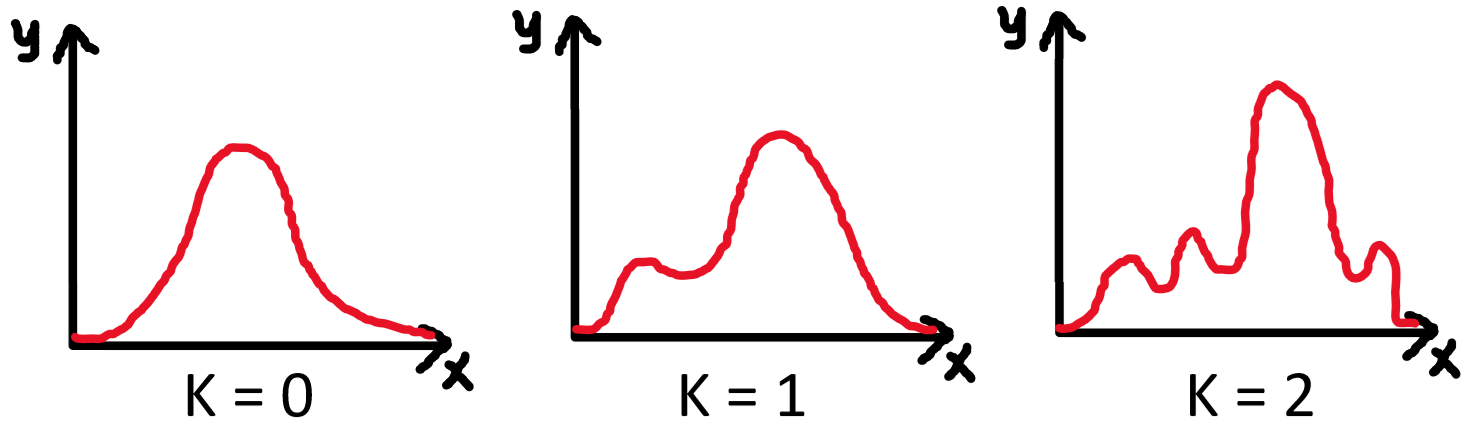
\includegraphics[width=0.8\textwidth]{images/simple_representation.PNG}
\caption{Simple 2-D representation on how a higher K increases the ruggedness of the function F()}
\end{figure}
\section{Algorithms}
To solve this problem we will use the mountain climbing algorithm, we will use the deterministic version as well as the probabilistic, we will see which one does better with higher K. The goal is to find an $x \in \{0,1\}^{N}$ that maximises $F(x)$.\\
Let's also define what is the neighbourhood of a point $x \in \{0,1\}^{N}$ as the algorithms will use it. The neighbourhood of a point $x \in \{0,1\}^{N}$ or $V(x)$ is defined by all the points $x' \in \{0,1\}^{N}$ at a hamming distance of 1 from $x$. The hamming distance between two strings of the same length, is the sum of different individual values, so 2 strings are of hamming distance 1, if only one bit between the two is different.
\subsection{Deterministic Hill-Climbing}
Lets see the a step by step analysis of the algorithm:
\begin{itemize}
\item[(1)] generate random $x \in \{0,1\}^{N}$
\item[(2)] compute the fitness of $x$ given by $F(x)$, let's call it $fit\_x$
\item[(3)] generate its neighbourhood or $V(x)$
\item[(4)] compute the fitness of all $x' \in V(x)$
\item[(5)] find the maximum fitness computed in step (4), and let's call it $fit\_x_{neighbor}$
\item[(6)] compare $fit\_x$ and $fit\_x_{neighbor}$
\begin{itemize}
\item[(6.a)] $fit\_x < fit\_x_{neighbor}$ $\longrightarrow$ we set x = neighbor with higher fitness and go back to step (2)
\item[(6.b)] $fit\_x \geq fit\_x_{neighbor}$ $\longrightarrow$ we return x as a maximum and finish the computation
\end{itemize}
\end{itemize}
In other words, at each step of the algorithm we look for the highest fit neighbor, and set it as the new x, if we don't find a higher fit neighbor, it means we are at a mountain top, so we stop the algorithm. We have to be ware that it might be a local maximum, and not at a global maximum.
\subsection{Probabilistic Hill-Climbing - with aspiration}
Lets see the a step by step analysis of the algorithm (some steps are the same as the deterministic version):
\begin{itemize}
\item[(1)] generate random $x \in \{0,1\}^{N}$
\item[(2)] compute the fitness of $x$ given by $F(x)$, let's call it $fit\_x$
\item[(3)] generate its neighbourhood or $V(x)$
\item[(4)] compute the fitness of all $x' \in V(x)$
\item[(5)] find the maximum fitness computed in step (4), and let's call it $fit\_x_{neighbor}$
\item[(6)] compare $fit\_x_{neighbor}$ and the best fitness ever seen during the computation $x\_fit\_best$
\begin{itemize}
\item[(6.a)] $x\_fit\_best < fit\_x_{neighbor}$ $\longrightarrow$ we set x = neighbor with higher fitness and go back to step (2)
\end{itemize}
\item[(7)] compute $total\_fitness$ the sum of all the fitness in the neighborhood, $total\_fitness = \sum_{x \in V(x)} F(x)$
\item[(8)] for every $x' \in V(x)$ compute $F(x')/total\_fitness$ from step (7), every neighbor has a normalised probability that is proportional to their own fitness
\item[(9)] use a probabilistic method from TP0 (roulette method), to chose randomly the next neighbor x depending on the probabilities computed in step (8), go back to step (2) with new x
\item[(stop)] we stop after a given number of 'rounds', and return the best ever x (we have to keep track of them) 
\end{itemize}
If we skip steps (5) and (6) we will have the Probabilistic Hill-Climbing algorithm without aspiration.
\subsection{Comment on the algorithms}
What changes between the 2 is the choosing of the next x, as the deterministic version always chooses the best neighbor possible, and the probabilistic version chooses randomly between the neighbors. Which means the probabilistic version might not get stuck in a local maximum, where the deterministic version will naively think it has done it's job perfectly while finding the local maximum.
\section{Results}
To try both algorithm's performances, we will create a random $x$ string of $N=21$ bits, making $\{0,1\}^{21}$ the search space, and use the algorithm with $K = \{0,1,2\}$. Since the result highly the depends on the first random $x$, we will run the same algorithm 50 times. To check how different the results were, we will compute the hamming distance between them.
\begin{figure}[H]
\center
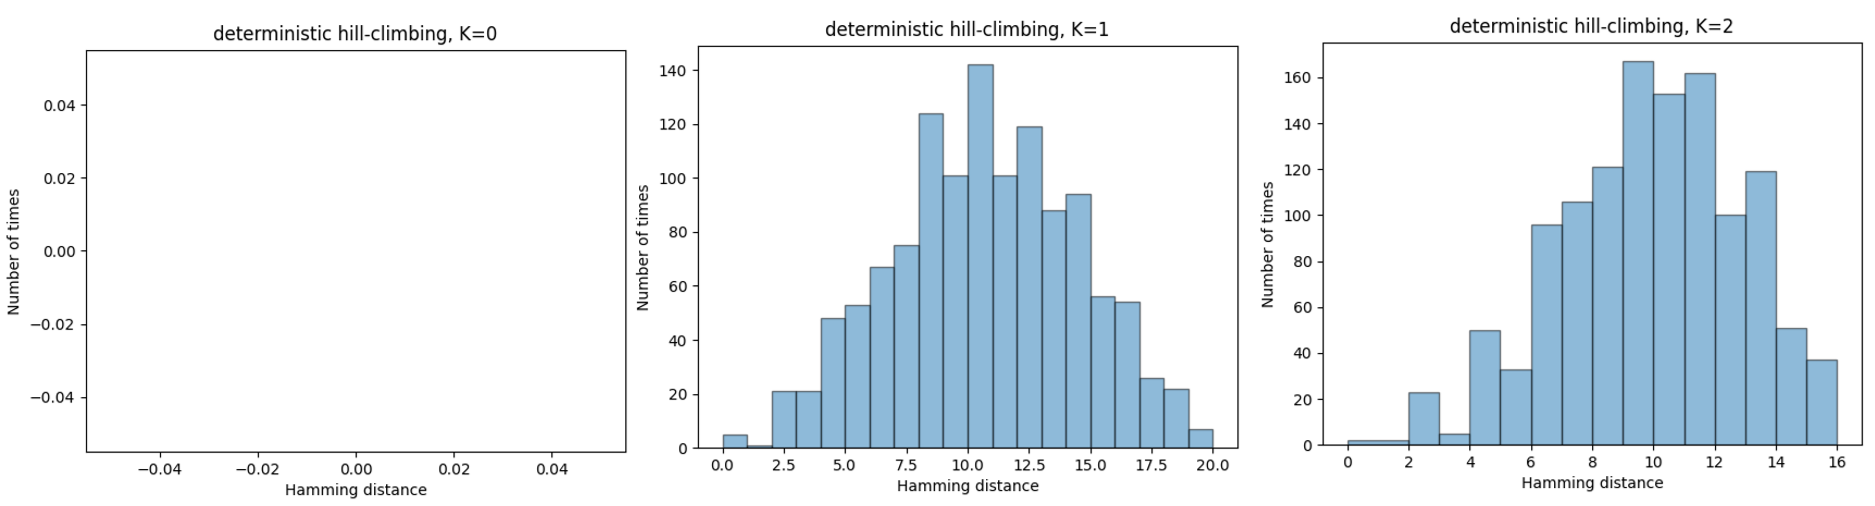
\includegraphics[width=1\textwidth]{images/hill_climb_deter.PNG}
\caption{Histogram representing the Hamming distance for deterministic hill-climbing $K=\{0,1,2\}$}
\end{figure}

\begin{figure}[H]
\center
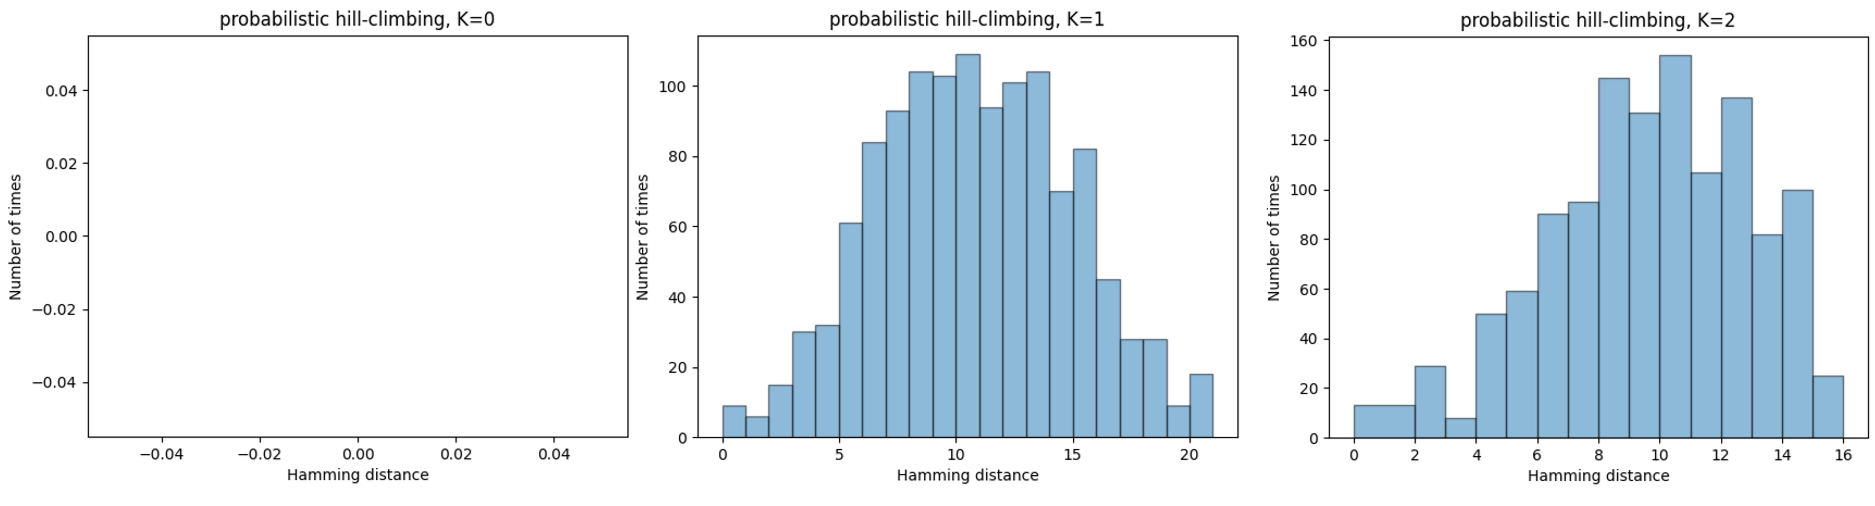
\includegraphics[width=1\textwidth]{images/hill_climb_proba.PNG}
\caption{Histogram representing the Hamming distance for probabilistic hill-climbing with aspiration $K=\{0,1,2\}$}
\end{figure}


Looking at figure 2 and 3, we can analyse how good both algorithms are, when $K=0$ both algorithms were able to find the global maximum every time. This is to be expected, the deterministic version only stops at a maximum, since there is only one maximum, it is easily found. The probabilistic variant with aspiration does have a deterministic side, as we make sure to explore a higher fitted $x$ if we've never seen one that is as good.\\

Looking at the other histograms in both figures, we can't see much difference between the two methods, as both of the graphs for a given K value show a similar gaussian. We can see that the bins are a bit more even in the probabilistic method, but it doesn't tell us that it is definitely better than the deterministic version.\\

To try and have a definitive idea of which method is best, we can plot the fitness of each returned $x$ by both methods with $K=\{1,2\}$

\begin{figure}[H]
\center
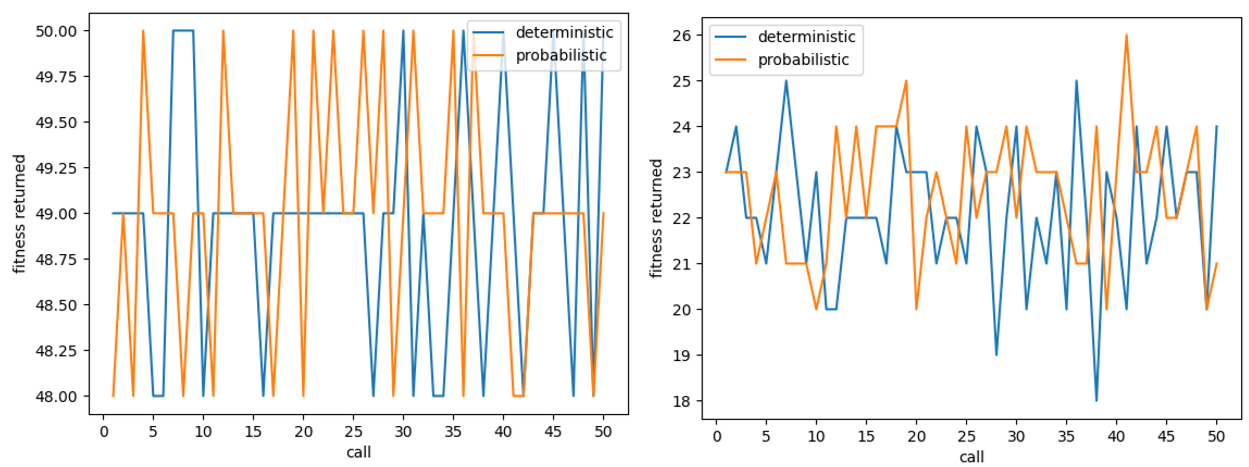
\includegraphics[width=1\textwidth]{images/proba_vs_deter.PNG}
\caption{Graphs representing the fitness of the $x$ returned by both algorithms, $K=\{0,1,2\}$}
\end{figure}
For K=1 we can see that both methods returned the same results, the same amount of real maximums, and the same amount of local maximums. Where it gets interesting, is with K=2, where we see that the deterministic could never achieve the global maximum.
\end{document}
